\documentclass[12pt]{article}
\usepackage{a4} 
\usepackage{hyperref} 
\usepackage{color}
\usepackage{graphicx} 
\usepackage{fancyhdr}
\usepackage{amssymb,amsmath}
\usepackage{bm}
\usepackage[lofdepth,lotdepth]{subfig}

\relpenalty=10000
\binoppenalty=10000

% Set page size:

\textwidth 160mm 
\textheight 235mm 
\oddsidemargin 0mm 
\topmargin -15mm
\baselineskip 13pt
\parskip 0pc 
\parindent 1pc

% Headers and footer using fancyhdr:

\definecolor{darkred}{rgb}{0.80,0.00,0.05}
\definecolor{blue}{rgb}{0.00,0.00,0.95}
\definecolor{darkgreen}{rgb}{0.00,0.60,0.0}
\definecolor{gray}{rgb}{0.95,0.9,0.9}

\title{Theoretical and Numerical Study of Models of Entanglement for
  Neutrons}

\date{14 May, 2012} 

\author{ Candidate Number: 8221T \\ Supervisor: Dr Crispin Barnes }

\begin{document} 

\maketitle

\begin{abstract}

We propose and investigate a scheme for detecting gravitational waves
using the entanglement generated by the dynamics of a pair of neutrons
trapped in a harmonic well. We develop a model that combines the
effects due to plane gravitational wave solutions of the linearised
field equations in the weak-field limit of general relativity with the
time-dependent Schr\"{o}dinger equation. Numerical simulations show
that entanglement amplifies the effect of high frequency gravitational
waves on the quantum state. In the proposed experiment, for realistic
wave amplitudes and frequencies, the final state is practically
indistinguishable from one unaffected by gravitational
radiation. However, the results also show that quantum entanglement
could be used in the future for high frequency gravitational wave
detection.

\end{abstract}


\section{Introduction}

A significant amount of experimental effort has gone into detecting
gravitational waves since the 1960s. They were first predicted by
Einstein in 1916 as a consequence of general relativity. Mass (or
energy) warps spacetime and changes in the shape or position of such
objects will cause distortions which propagate as waves at the speed
of light. Gravitational waves have still not been observed
directly. However, the study of the period of the binary pulsar
discovered by Hulse and Taylor in 1974 provides strong indirect
evidence for their existence \cite{pulsar}. The search for direct
evidence of gravitational waves has resulted in a number of
large-scale experiments such as the Laser Interferometer
Gravitational-Wave Observatory (LIGO) and the Laser Interferometer
Space Antenna (LISA). The main difficulty of direct detection of
gravitational radiation is its small effect on a detector, distortions
from equilibrium on Earth due to astrophysical sources are predicted
to be no larger than one part in $10^{21}$ \cite{hobson}. To observe
such a small effect an extremely sensitive apparatus is necessary. The
LIGO and LISA experiments use laser interferometry as a means to
detect such tiny changes. However, the fragile nature of entanglement
could provide an alternative for an experiment to detect this effect.

Entanglement, a phenomenon unique to quantum mechanics, allows for
stronger correlations between separate components of a composite
system than are possible with classical statistics. This ``spooky
action at a distance'' led Einstein to dismiss the theory as an
incomplete description of reality \cite{epr}. However, in 1964 John
Bell showed that no physical theory of local hidden variables, as
suggested by Einstein, can reproduce the predictions of quantum
mechanics. A number of experiments have been performed to test Bell's
theorem and all of them provide strong evidence for the validity of
quantum mechanics. The first definitive experiment was performed by
Alain Aspect in 1982 \cite{aspect}.

Experiments have shown that quantum entanglement is not only real, but
that it can also be used as a resource. The idea that it can be
generated and manipulated like any other physical property of a system
gave rise to the field of quantum information. Entanglement has
allowed us to exceed limits imposed by classical mechanics in
computing, cryptography and data transmission \cite{steane}. However,
in reality quantum entanglement is a fragile resource which is very
difficult to control. Decoherence, the loss of quantum coherences due
to coupling to the environment, occurs on time scales much shorter
than the rate at which we can manipulate the systems experimentally
\cite{zurek}. This sensitivity to environmental effects is one of the
main obstacles in developing quantum technologies and is a subject of
active research. However, this fragility could potentially be used to
measure very small effects that require extremely sensitive
detectors. 

We propose and investigate numerically the possibility of performing
an experiment to detect gravitational waves using the entanglement
between a pair of neutrons initially localized on either side of a
harmonic potential in a multilayer. Entanglement is generated in
collisions due to the particles' natural motion \cite{edmund}. By
working in the weak-field limit of general relativity we combine the
effect of gravitational waves with the Schr\"{o}dinger equation. The
resulting equation is then investigated numerically and we demonstrate
that entanglement amplifies the effect of a gravitational wave, but
the effect is too small to detect using conventional, easily
accessible techniques originally envisaged for this
experiment. However, the results show that entanglement can be a
useful mechanism for detecting high frequency waves.

In section \ref{sec:experiment}, we present the experimental setup
that will be investigated and the mechanism for entanglement
generation. In section \ref{sec:model}, we describe the effect of
gravitational waves, the neutron-neutron interaction and how these
elements are combined in a two-particle Hamiltonian. We also address
various concerns that arise when combining general relativistic
effects with quantum mechanics. Section \ref{sec:numerical} presents
the numerical simulations of the modified Schr\"{o}dinger equation and
their implications for the feasability of the suggested experiment. We
conclude in section \ref{sec:conclusions}.



\section{The Experiment}\label{sec:experiment}

\subsection{Gravitational Waves}

The strength of gravitational radiation on Earth from typical
astrophysical sources is very small. The largest strains one might
expect to measure are of order $10^{-21}$ \cite{hobson}. Therefore, we
make the physical assumption that the gravitational fields are
weak. Mathematically this corresponds to linearising the gravitational
field equations. The basic mathematical framework of gravitational
waves in linearised general relativity is summarised in appendix
\ref{sec:appendix}. It is possible to choose a gauge in which the
coordinate separation between the particles is constant at all times,
but this has no coordinate-invariant physical \mbox{meaning
\cite{hobson}}. However, the physical spatial separation $l$, which is
given by $l^2 = -g_{ij}\xi^i\xi^j$, will vary since the metric tensor
components are not constant in the presence of a gravitational
wave. The effect of a single passing gravitational wave on a cloud of
non-interacting test particles is illustrated in figure
\ref{fig:rings}.

\begin{figure}[htbp]
  \begin{center}
    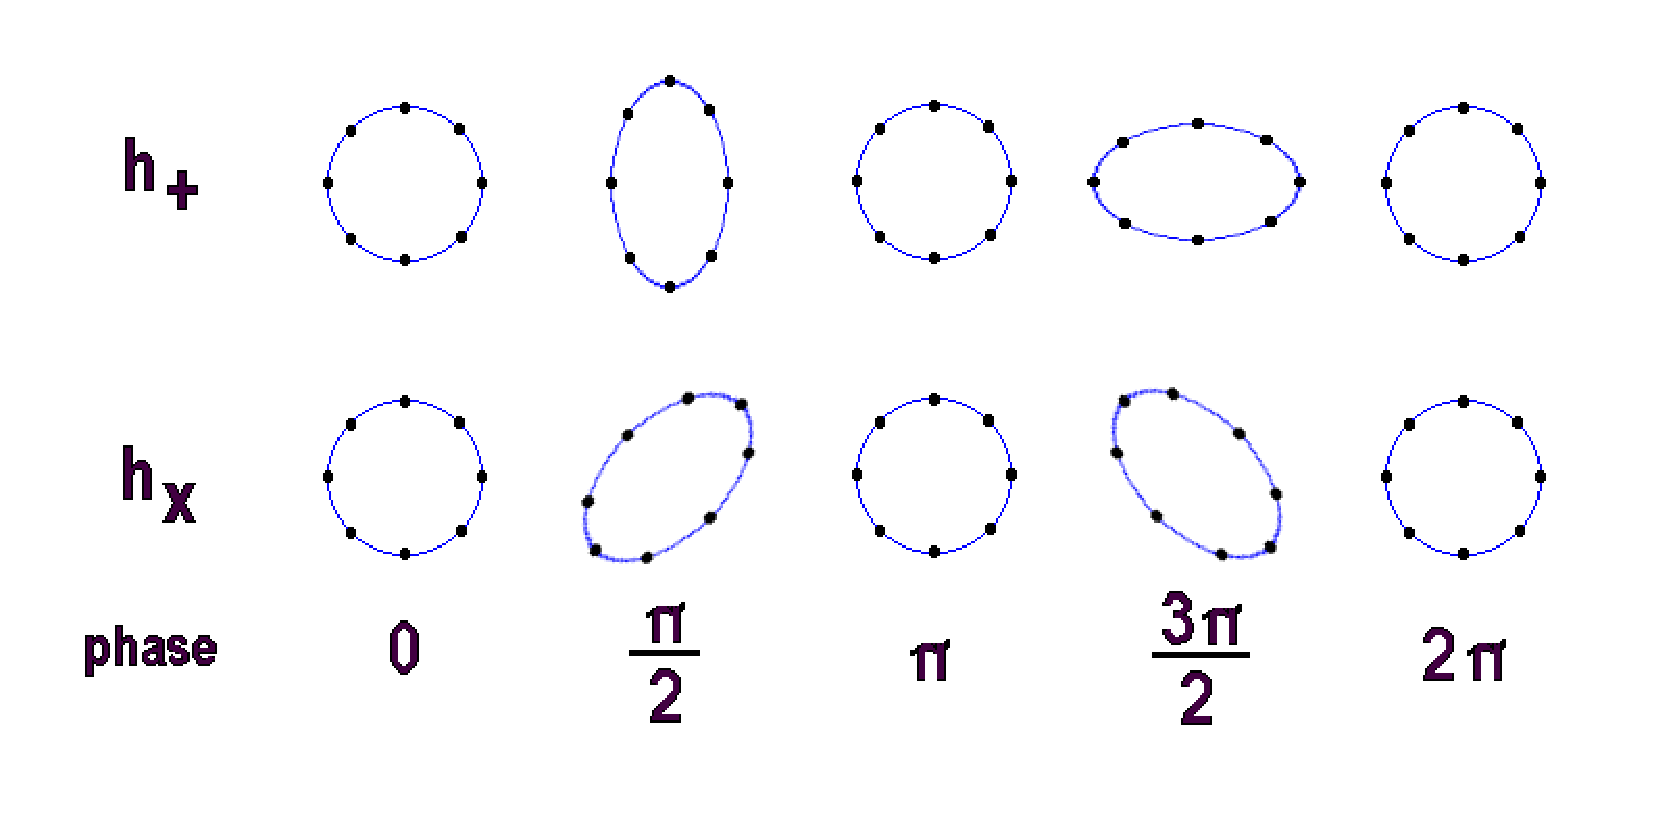
\includegraphics[width=150mm]{Images/rings.pdf}
    \caption{\label{fig:rings} The effect of a passing gravitational
      wave on a circle of test particles. The two different
      polarisations are at $45^\circ$ to each other. Figure reproduced
      with permission \cite{rings}.}
  \end{center}
\end{figure}

\subsection{The Experimental Setup}

We consider a one-dimensional system where the two neutrons with
opposite spins interact in a quantum harmonic oscillator. The two
particles are introduced in coherent states at rest on either side of
the potential. They will oscillate in the harmonic trap, interact and
eventually tunnel out. Repeating this experiment several times for the
same initial condition will reveal information about the state and
entanglement generated within the multilayer. If all unwanted effects
are reduced to acceptable levels then the results will depend on the
presence of gravitational waves if they have an effect on the
entanglement of the two neutrons.

Such a trap can be constructed using a multilayer of ultrathin
magnetic films of suitably chosen materials using molecular beam
epitaxy. The detailed behaviour of neutrons in such multilayers is
presented in \cite{blundell} where polarized neutron reflection was
used to study the magnetic properties of thin films. The potential
energy in the $\alpha$th region can be written as a sum of a nuclear
and magnetic term
\begin{equation}\label{eq:pot}
V_\alpha = \frac{\hbar^2}{2\pi m_n}\rho_\alpha b_\alpha -
\boldsymbol{\mu_n}\cdot\boldsymbol{B_\alpha},
\end{equation}
where $\boldsymbol{\mu_\alpha}$, $b_\alpha$, $\boldsymbol{B_\alpha}$
and $\rho_\alpha$ are the neutron moment, coherent nuclear scattering
length, magnetic field due to the magnetization in the region and
atomic density, respectively. The harmonic oscillator potential itself
can be formed from layers with no magnetization as long as the
thickness of a single film is much less than the particle wavelength
so the discrete nature of the material can be ignored. The second term
in \eqref{eq:pot} leads to different values for the potential
depending on the orientation of the neutron's spin relative to the
magnetic field. Hence, we can use magnetized layers as spin dependent
barriers. By placing such barriers at the two ends of the trap we
provide means for a spin measurement.

It has been shown that under certain approximations the quantum
dynamics of such a system are sufficient to generate maximally
entangled states under appropriate conditions \cite{edmund}. Producing
maximally entangled states with high fidelity is not necessary in this
experiment, but the work by Owen et al. provides a useful framework to
describe and model the entanglement in a harmonic trap.

The two particles are initialized separately such that their single
particle wave functions are spatially distinct at $t = 0$. We consider
neutrons, mass $m$, in a harmonic potential of the form $V =
\frac{1}{2}m \omega^2x^2$ initially in the coherent states
$\psi_{L/R}(x)$, where
\begin{equation}
\psi_R = A\exp\left( -\frac{m\omega}{2\hbar}(x - x_0)^2 \right) ,
\end{equation}
\begin{equation}
\psi_L(x) = \psi_R(-x),
\end{equation}
$x_0 > 0$ and $A$ is a normalization constant. To be spatially distinct, the
single particle wave functions must satisfy $\int_{-\infty}^0 \! \psi_R(x) \,
\mathrm{d} x \to 0$ and $\int^{\infty}_0 \! \psi_L(x) \, \mathrm{d} x
\to 0$. We can then write the initial two-particle state as
\begin{equation}
\begin{array} {lcl}
|\Psi(t=0)\rangle & = & \left( \int \!
\psi_L(x_1)a^\dagger_{\sigma_1}(x_1) \, \mathrm{d} x_1 \right) \left(
\int \! \psi_R(x_2)a^\dagger_{\sigma_2}(x_2) \, \mathrm{d} x_2 \right)
|0\rangle \\\\ & \equiv & \left( \int\int\Psi(x_1, x_2;
t=0)a^\dagger_{\sigma_1}(x_1)a^\dagger_{\sigma_2}(x_2) \mathrm{d} x_1
\mathrm{d} x_2 \right) |0\rangle \\\\ & \equiv &
|L_{\sigma_1}R_{\sigma_2}\rangle
\end{array}
\end{equation}
where $a^\dagger_{\sigma_i}(x_i)$ are the creation operators for a
neutron at $x_i$ with spin $\sigma_i$. We only consider neutrons which
are introduced into the trap with opposite spins, $\sigma_1 \neq
\sigma_2$, hence we can treat them as distinguishable. Therefore, the
creation operators commute.

The two-particle Hamiltonian for the two neutrons in the same harmonic
potential is given by
\begin{equation}\label{eq:hamiltonian}
\hat{H} = -\frac{\hbar^2}{2m}\left( \frac{\partial^2}{\partial x_1^2}
+ \frac{\partial^2}{\partial x_2^2} \right) +
\frac{1}{2}m\omega^2(x_1^2 + x_2^2) + V_{nn}(x_1-x_2)
\end{equation}
where $V_{nn}(x_1-x_2)$ is a translationally invariant potential between
the two neutrons and its exact form will be discussed in the next
section.

In the parity-dependent harmonic approximation, which assumes that the
spectrum of the Hamiltonian in \eqref{eq:hamiltonian} is equal to the
spectrum of a quantum harmonic oscillator except for a
parity-dependent energy shift, the wave function at integer
half-periods has been shown to be
\begin{equation}
|\Psi(t=n\pi/\omega)\rangle \propto
\cos\theta|L_{\sigma_1}R_{\sigma_2}\rangle +
e^{i\chi}\sin\theta|R_{\sigma_1}L_{\sigma_2}\rangle,
\end{equation}
where $\theta = n\pi\phi/2$, $\phi\hbar\omega$ is the energy shift
to the even parity eigenstates and $\chi$ is some phase \cite{edmund}.



\section{The Model}\label{sec:model}

\subsection{Gravitational Waves}

Any reasonable signal possible to detect on Earth will be of
astrophysical origin. Hence, we can assume that the source is far
enough to treat the waves as plane waves. Therefore, in order for our
model to be able to account for several gravitational waves we have to
expand the formalism for the plane wave solutions presented in
appendix \ref{sec:appendix} to a superposition of multiple waves. We
adopt the viewpoint that $h_{\mu\nu}$ is a symmetric tensor field
(under global Lorentz transformations) defined in quasi-Cartesian
coordinates on a flat Minkowski background spacetime. Since we work
with linearised general relativity we can easily obtain the solution
by superposing the single plane wave solutions
\begin{equation}\label{eq:manywaves}
\bar{h}^{\mu\nu} = \sum_j(A_j)^{\mu\nu}\exp(i(k_j)_\rho x^\rho),
\end{equation}
where $A_j^{\mu\nu}$ are constant components of symmetric tensors and
$(k_j)_\mu$ are the constant, real components of vectors. We assume the
summation convention, but explicitly state the summation over the
index $j$ as it does not run over the coordinate indices, but over all
plane waves present.

We consider a guage transformation of the same form as the transverse
traceless gauge used in appendix A which is defined as
\begin{equation}\label{eq:manyTT}
\bar{h}^{0a}_{TT} \equiv 0 \,\,\,\,\,\, \text{and} \,\,\,\,\,\, \bar{h}_{TT} \equiv 0,
\end{equation}
where latin alphabet indices run over the spatial dimensions
only. Furthermore the Lorenz gauge condition gives the constraints
\begin{equation}
\partial_0\bar{h}^{00}_{TT} = 0 \,\,\,\,\,\, \text{and} \,\,\,\,\,\, \partial_a\bar{h}^{ab}_{TT} = 0.
\end{equation}
Whilst we cannot consider this gauge to be transverse anymore since we
are considering waves travelling in different directions, we will keep
the labels since we are using exactly the same definition. This
generalisation is straightforward, because of the linear nature of the
field equations in a weak gravitational field. The field tensor
transforms as 
\begin{equation}\label{eq:transformation}
\bar{h}^{\mu\nu}_{TT} = \bar{h}^{\mu\nu} - \partial^{\mu}\xi^{\nu} -
\partial^{\nu}\xi^{\mu} + \eta^{\mu\nu}\partial_\rho\xi^\rho,
\end{equation}
where $\xi^\mu$ are four functions that define the gauge
transformation and which must satisfy $\Box^2\xi^\mu$ to preserve the
Lorenz gauge. The solution in \eqref{eq:manywaves} is a linear
superposition of waves with different wavevectors and Each of the
components can be transformed into the TT gauge using some set of
functions $\xi^\mu_j$ (see appendix \ref{sec:appendix} for
details). Therefore, we can transform \eqref{eq:manywaves} using
$\xi^{\prime\mu} = \sum_j \xi^\mu_j$ since the transformation
\eqref{eq:transformation} is linear in $\xi^\mu$. Applying this
transformation gives us the same constraints on the constant
$A_j^{\mu\nu}$ components separately for all values of $j$. Therefore
in the new gauge the coefficients must satisfy
\begin{equation}
(A_j)^{0a}_{TT} = 0 \,\,\,\,\,\, \text{and} \,\,\,\,\,\, ((A_j)_{TT})^\mu_\mu = 0
\end{equation}
and the Lorenz gauge conditions require that
\begin{equation}
(A_j)^{00}_{TT} = 0 \,\,\,\,\,\, \text{and} \,\,\,\,\,\, (A_j)^{ab}_{TT}k_b = 0.
\end{equation}
Using these conditions we can construct a traceless tensor which
satisfies the definition in \eqref{eq:manyTT}. It is a superposition
of waves of the form \eqref{eq:manywaves}
\begin{equation}\label{eq:manyh}
\bar{h}^{\mu\nu}_{TT} = \sum_j(A_j)_{TT}^{\mu\nu}\exp(i(k_j)_\rho x^\rho),
\end{equation}
where $(A_j)_{TT}^{0\mu} = (A_j)_{TT}^{\mu 0} = 0$, the spatial
components are given by
\begin{equation}
(A_j)^{ab}_{TT} = ((P_j)^a_c(P_j)^b_d - \frac{1}{2}(P_j)^{ab}(P_j)_{cd})(A_j)^{cd},
\end{equation}
$(P_j)_{ab} \equiv \delta_{ab} - (n_j)_a(n_j)_b$ and $(n_j)_a =
(\hat{k}_j)_a$.

\subsection{Neutron-neutron Interaction}

Nucleon-nucleon scattering is fundamentally a many body problem
governed by quantum chromodynamics. However, the strong interaction
has a very short range ($\sim$ a few fm) and $kR \ll 1$, where $k$ is
the neutron wave vector and $R$ the range of the potential. This means
that we only have to consider s-wave scattering and we can approximate
the scattering potential with a delta function $V_{nn} =
U\delta(\vec{r}_1 - \vec{r}_2)$. To obtain the value of $U$ we use the
fact that for s-wave scattering the cross-section is given by $\sigma
= 4\pi a_s^2$, where $a_s$ is the scattering length which can be
measured experimentally. Therefore, in the Born approximation we
obtain
\begin{equation}\label{eq:nn}
U = \frac{2 \pi a_s \hbar^2}{m_n},
\end{equation}
where $m_n$ is the mass of the neutron. Gravitational waves cause the
distance between the two neutrons, $|\vec{r}_1 - \vec{r}_2|$, to
oscillate. However, because the inter-particle interaction is in the
form of a contact potential it remains unaffected in the presence of a
passing wave. The physical spatial separation will only be zero if the
coordinate separation vector will also be zero.

\subsection{The Schr\"{o}dinger Equation}

The gravitational wave background is predicted to have no significant
components at wavelengths shorter than a few km which is much larger
than the lengthscales we are considering for the
experiment. Therefore, combined with the fact that we are only
considering weak gravitational fields, we can assume that in order to
model the effect of gravitational waves on the quantum state of two
neutrons in a harmonic trap we do not need to resort to a full quantum
description of the interaction.

In order to incorporate the effect of passing waves on the quantum
state we begin by considering the two-particle Schr\"{o}dinger
equation for the Hamiltonian given in \eqref{eq:hamiltonian}
\begin{equation}\label{eq:schrodinger}
i\hbar\frac{\partial \Psi(x_1, x_2; t)}{\partial t} = \left[
  -\frac{\hbar^2}{2m}\left( \frac{\partial^2}{\partial x_1^2} +
  \frac{\partial^2}{\partial x_2^2} \right) +
  \frac{1}{2}m\omega^2(x_1^2 + x_2^2) + V_{nn}(x_1-x_2)
  \right]\Psi(x_1, x_2; t).
\end{equation}
We have already shown that the form of $V_{nn}$ is unaffected. The
potential due to the interaction with the harmonic trap also remains
unchanged as it does not depend on the physical separation between two
points. A huge benefit of the gauge we have chosen to work in is the
fact that only the spatial components of the metric are affected by
the gravitational wave which means that the time derivative on the
left hand side does not have to be modified. Only the spatial
derivatives have to be considered in this situation.

For a general metric the Laplacian of a scalar field is given by
\begin{equation}\label{eq:laplacian}
\nabla^2\phi = \frac{1}{\sqrt{|g|}}\partial_a \left( \sqrt{|g|} g^{ab}
\partial_b\phi \right),
\end{equation}
where $g$ is the determinant of the metric tensor which in the TT
gauge, to first order in $h$, is equal to unity. We now want to reduce
the problem to only one spatial dimension to simplify the model. As
this is only an investigation into the feasibility of such an
experiment such a simplification is desirable as it reduces the
necessary computational time required to obtain qualitatively the same
results. The gravitational waves are very weak so we assume that
confinement in the $y$ and $z$ directions is strong enough that the
wavefunction remains in its ground state along those axes at all
times. This means that we can ignore all second derivative terms apart
from $\frac{\partial^2 \Psi}{\partial x^2}$ since this is the only
significant kinetic energy term. Furthermore, we will have terms of
the form $\partial_a g^{ab} \partial_b \phi$. These terms can also be
ignored, because $\partial_a g^{ab} \propto k_a$ and for any realistic
setup the wavelength of the waves will be much larger than the size of
the expriment making these terms insignificant. Therefore the only
relevant terms that we are left with are
\begin{equation}\label{eq:kinetic}
\nabla^2 \Psi = g^{xx}\frac{\partial^2 \Psi}{\partial x^2},
\end{equation}
where the effective form of $g^{xx}$ is obtained from \eqref{eq:manyh}
\begin{equation}
g^{xx} = 1 + \sum_i A^{xx}_i \cos(\Omega_i t + \phi_i),
\end{equation}
$\Omega_i$ is the frequency of the $i$th wave, $\phi_i$ is the $i$th
wave's phase at $x=0$ and we have ignored phase variation along the
trap axis, $k_x x$, since we consider wavelengths much larger than the
dimensions of the well.

The most general form of the one-dimensional Laplacian in the TT gauge
that preserves probability when used in the Sch\"{o}dinger equation is
\begin{equation}\label{eq:general}
\nabla^2 \Psi = g^{xx}\frac{\partial^2 \Psi}{\partial x^2} +
\frac{\partial g^{xx}}{\partial x} \frac{\partial \Psi}{\partial x}.
\end{equation}
This imposes some additional restrictions on the components of the
metric tensor. We again ignore second derivative terms due to
confinement along the other axes. However, we must now require $g^{xy}
= g^{xz} = 0$ for equation \eqref{eq:general} to be correct. In order
to investigate gravitational waves with shorter wavelengths we want to
be able to use this equation for the Laplacian. However, under the TT
and Lorenz gauge conditions the additional constraints also require
$g^{xx} = 0$ unless the wavevectors are perpendicular to the
$x$-axis. This in turn implies $\partial_x g^{xx} = 0$ since $k_x =
0$. Therefore, in our investigation we always use equation
\eqref{eq:kinetic}, but for wavelengths comparable to or smaller than
the trap dimensions this limits us to the study of waves perpendicular
to the $x$-axis.

Neutrons are spin-$\frac{1}{2}$ particles and so also we have to
address the question of how the intrinsic angular momentum of the
particles couples to the gravitational waves. The theoretical
possibility of such coupling was first considered by Kobzarev and Okun
in 1963 \cite{kobzarev}. If we consider a Newtonian gravitational
potential $\phi$ then the coupling to spin would take the form
$H_{int}=A\vec{\sigma}\cdot\nabla\phi$, where $A$ is an amplitude
and $\vec{\sigma}$ is the particle spin. However, this violates the
equivalence principle which states that the trajectory of a point mass
in a gravitational field depends only on its initial position and
velocity, and is independent of its composition. Therefore, we do not
have to take into account any spin-gravity coupling since we are
working in the weak field limit.

The final form of the two-particle Hamiltonian that we
will be investigating is
\begin{equation}\label{eq:main}
\hat{H} = - g^{xx} \frac{\hbar^2}{2m} \left(
  \frac{\partial^2}{\partial x_1^2} + \frac{\partial^2}{\partial
    x_2^2} \right) + \frac{1}{2}m\omega^2(x_1^2 + x_2^2) +
V_{nn}(x_1-x_2).
\end{equation}



\section{Numerical Simulations}\label{sec:numerical}

We want to study the effect of gravitational waves on the entanglement
and distinguishability of the final state from one unaffected by the
radiation. The von Neumann entropy of entanglement,
\begin{equation}
S = -\text{Tr}(\rho_1 \log_2 \rho_1) = -\text{Tr}(\rho_2 \log_2
\rho_2),
\end{equation}
where $\rho_i$ is the reduced density matrix of particle $i$, is a
standard measure of entanglement of two particles. The fidelity of
quantum states is a suitable measure of their distinguishability. It
is given by
\begin{equation}
\mathcal{F} = | \langle \psi_0 | \psi_{gw} \rangle |,
\end{equation}
where $| \psi_{gw} \rangle$ is the state calculated in the presence of
a gravitational wave background and $| \psi_0 \rangle$ is the state
calculated in their absence. $\mathcal{F}^2$ is then just the
probability of observing the outgoing particle in the state predicted
for a flat spacetime and will always be equal to unity if $| \psi_{gw}
\rangle = | \psi_0 \rangle $.

\begin{figure}[htbp]
  \begin{center}
    \subfloat[][\label{fig:HighFreq}]{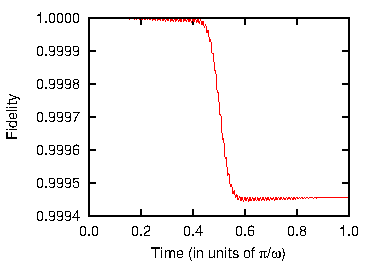
\includegraphics[width=75mm]{Images/HighFreq.pdf}}
    \qquad
    \subfloat[][\label{fig:LowFreq}]{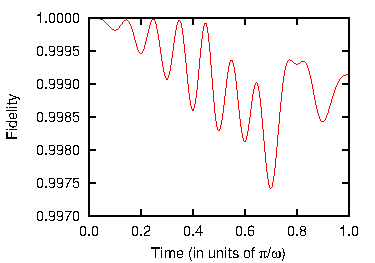
\includegraphics[width=75mm]{Images/LowFreq.pdf}}
    \caption{\label{fig:Fidelity} Fidelities of the wavefunction in
      the presence of a single gravitational wave at different
      frequencies to the unaffected state. \subref{fig:HighFreq}
      $\Omega = 100\omega$. The large drop at $t=\pi/\omega$ is
      evidence that interaction enhances the effect of the
      gravitational waves. \subref{fig:LowFreq} $\Omega =
      10\omega$. We see no evidence of interaction at $t=\pi/\omega$
      as it has no effect in this regime. }
  \end{center}
\end{figure}

We can distinguish two regimes for gravitational waves interacting
with a two particle quantum system in a harmonic trap based on their
relation to the interaction time, $\tau$, which is the length of time
during which the wave packets overlap is significant. Firstly, there
are high frequency waves for which $\Omega \gg \tau^{-1}$. Figure
\ref{fig:HighFreq} shows the evolution of fidelity over a single
collision for a single wave of frequency $\Omega = 100 \omega$. The
biggest change in fidelity occurs during the collision itself when the
wave packets overlap, interact and entangle. Outside the collision,
when the overlap is small the fidelity simply oscillates with an
amplitude that increases with the particle's speed. We clearly see
that the effect of the gravitational wave is amplified in the
interaction which leads to a permanent change in the value of
$\mathcal{F}$. The change in fidelity is dominated by the change in
the entanglement of the two particles due to the radiation. The low
frequency regime is defined as $\Omega \ll \tau^{-1}$. Figure
\ref{fig:LowFreq} clearly shows that such waves have a larger effect
on the fidelity, but it is independent of the interaction. This effect
is classical and the low fidelity is due to a change of the classical
trajectory and final position of the particle in the harmonic
potential. We will not consider low frequency waves in this
investigation anymore since if we were intending on studying such
waves we would not need to resort to a quantum mechanical model to
describe their effect on the particles.

We see from figure \ref{fig:Freqs} that the high frequency regime
begins beyond $10 \omega$ as the inter-particle interaction starts
having a visible effect on the fidelity of the final state. These
results show that entanglement may be more useful in detecting high
frequency gravitational waves rather than a general stochastic
background since the effect of lower frequencies, which affect the
classical behaviour of the system, are much larger. Figure
\ref{fig:Freqs} shows that in the high frequency regime the quantum
effect of the waves on the fidelity can be even $10^6$ larger than the
effect due to the change in the classical trajectory. This
amplification is likely to be even stronger for higher frequencies
when we would no longer be able to ignore the first derivative terms
in equation \eqref{eq:laplacian}. Unfortunately, the gravitational
wave background is predicted not to have any significant components
above \mbox{100 kHz}, which will usually be smaller than or comparable
to the value of $\omega$ for a multilayer trap. Therefore,
entanglement is not a very useful mechanism for detecting background
radiation.

\begin{figure}[htbp]
  \begin{center}
    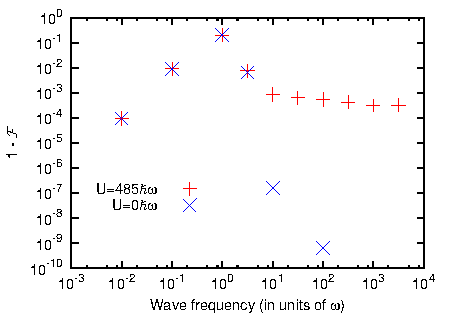
\includegraphics[width=120mm]{Images/Freqs.pdf}
    \caption{\label{fig:Freqs} The fidelity change of the wavefunction
      in the presence of a single gravitational wave to an unaffected
      state for two different interaction strengths. We observe
      resonance at $\omega$ which is in the classical low frequency
      regime. The interplay between the gravitational waves and
      entanglement begins beyond $\Omega = 10 \hbar \omega$.}
  \end{center}
\end{figure}

Figure \ref{fig:EntanglementSingle} shows the von Neumann entropy of
entanglement for a single collision. The form of the entropy does not
change at all as a function of gravitational radiation. However, its
final value does vary in the presence of waves, but the effect is very
small compared to the change due to the particle dynamics in the
collision itself. In the high frequency regime the waves' effect on
the entanglement is larger than their effect on the trajectories of
the particles, therefore, the fidelity of the final state to the
unaffected wavefunction is a better measure of the change in
entanglement of the system than entropy itself.

\begin{figure}[htbp]
  \begin{center}
    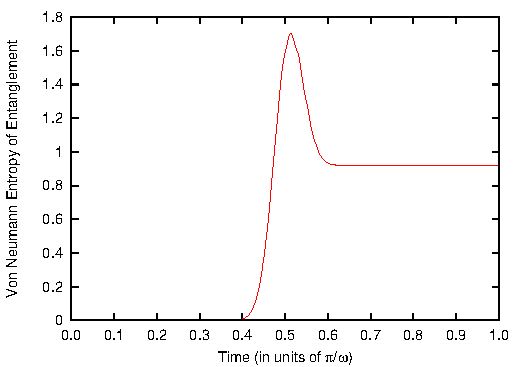
\includegraphics[width=120mm]{Images/EntanglementSingleWave.pdf}
    \caption{\label{fig:EntanglementSingle} The von Neumann entropy of
      entanglement of the wavefunction in the presence of a single
      gravitational wave. Oscillations are present, but they are
      significantly smaller than the change in entropy due to the
      interaction.}
  \end{center}
\end{figure}

The values of the $S$ and $\mathcal{F}$ are plotted over a suitable
range of interaction strengths in figure \ref{fig:Uplot} for a single
high frequency wave. Whilst the largest change in fidelity does not
coincide with the case where the final state is maximally entangled,
the fidelity changes the most when entanglement is produced. This
suggests that the amplification of the effect is due to the wave's
influence on the system's entanglement. Following the fidelity and von
Neumann entropy for multiple collisions confirms the correlation
between fidelity and entropy. The dynamics of particles will cause the
entanglement to increase and decrease during the collisions and the
change in fidelity follows the same trend.

\begin{figure}[htbp]
  \begin{center}
    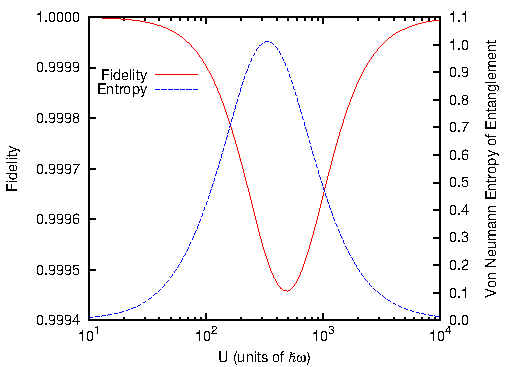
\includegraphics[width=120mm]{Images/Uplot.pdf}
    \caption{\label{fig:Uplot} The values of the von Neumann entropy
      of entanglement and fidelity of the state affected by waves to
      the unaffected state after a single collision. Entanglement
      amplifies the effect of the gravitational wave on the
      wavefunction, but the maximum value of entropy does not coincide
      with the minimum value of fidelity.}
  \end{center}
\end{figure}

To compare the effects of different radiation strengths on the quantum
state we define the intensity of the signal to be $I = \sum_j
(A^{xx}_j)^2$ which is proportional to the energy flux of the wave
\cite{hobson}. All of the results produced so far were calculated for
the largest possible value, $I = 0.01$. Higher intensities are not
investigated since in those cases the weak field approximation is no
longer valid. However, simulating realistic values of strain is beyond
even machine double precision. In order to estimate the size of the
effect of gravitational waves on the quantum state the value of
fidelity is evaluated for different intensities that are within
machine precision. The results in figure \ref{fig:WaveMags} show that
the change in the final value of fidelity is proportional to the
intensity of the waves. This is a very useful relationship as it lets
us easily estimate the size of the gravitational waves' effect for
different intensities. The square of the fidelity $\mathcal{F}^2$ is
just the probability of observing the final state to be that predicted
for a flat spacetime. Therefore, if we measure the final state
(e.g. by measuring the spin of outgoing neutrons) several times then
on average $1 - \mathcal{F}^2$ of the time we should obtain a
different result than predicted by the dynamics of the particles alone
in the absence of radiation. From the results in figure
\ref{fig:WaveMags} we find that $1 - \mathcal{F} = 0.5I$. Therefore,
the probability, $p$, of measuring a different state than expected can
be shown to be
\begin{equation}\label{eq:prob}
p = 1 - \mathcal{F}^2 \approx I.
\end{equation}
Different wave combinations will lead to different numerical
prefactors as the relationship between $1 - \mathcal{F}$ and $I$ is
linear regardless of the frequency regime and number of waves. The
highest intensity we can investigate in the weak field limit and high
frequency regime gives $p=0.01$. This is a small value, but
potentially measurable. However, extrapolating to the expected
detectable values of strain gives $p \approx 10^{-40}$. Assuming
Poissonian statistics in the spin counting process this requires
$\sim10^{27}$ measurements in order to make the error smaller than the
signal which shows that such an experiment is impractical.

\begin{figure}[htbp]
  \begin{center}
    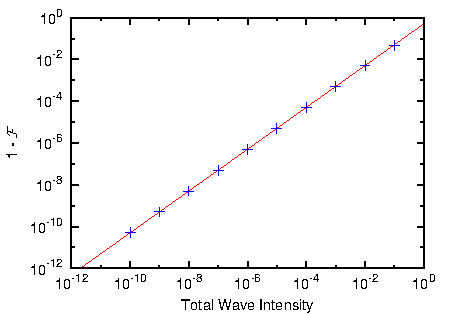
\includegraphics[width=120mm]{Images/WaveMags.pdf}
    \caption{\label{fig:WaveMags} The change in fidelity $\Delta = 1 -
      \mathcal{F}$ plotted against the total intensity. This change is
      proportional to the total intensity $\Delta = 0.5I$ over a very
      large range of values. The relationship is linear regardless of
      the number of waves or the frequency components present. }
  \end{center}
\end{figure}

We can now answer the question whether gravitational waves can be
detected using neutrons in the suggested experiment. We have already
discussed the applicability of the proposed scheme to detecting the
gravitational wave background and concluded that the experiment's
frequency range is too high and the classical effect of low frequency
waves is much larger anyway. We have also shown that the probability
of measuring an effect due to gravitational waves scales linearly with
the wave intensity which means that for realistic wave amplitude
values we will observe a different state only $\sim 10^{-40}$ of the
time. Additionally, it can be shown that for typical multilayer
dimensions and potentials the value of the neutron interaction in
\eqref{eq:nn} will be $U \approx 10^7 \hbar\omega$ which corresponds
to a point beyond the plotted range in figure \ref{fig:Uplot}. This
means that two neutrons introduced in coherent states on either side
of the well will not entangle in the collision and hence the quantum
effect of even high frequency gravitational waves will be minimal. The
neutrons will simply bounce of each other and behave classically. The
most significant effect the waves have on such a system is to cause
the physical separation of the two particles to oscillate and in this
case two neutrons in a multilayer are not the most optimal system for
detecting gravitational waves.



\section{Conclusions}\label{sec:conclusions}

We have proposed and investigated the feasibility of an experiment to
detect gravitational waves using the entanglement of two neutrons
trapped in a harmonic well. The quantum dynamics of the two particles
lead to entanglement which is affected by the presence of
gravitational radiation. We have shown that entanglement amplifies the
effect of high frequency gravitational waves on the
wavefunction. However, for realistic values of the wave amplitudes the
effect is too small to be measured in a device with the dimensions of
a typical multilayer.

The effects of gravitational waves were combined with the quantum
dynamics of the two neutrons in the weak-field limit, where the
linearised field equation could be used. The effects of the
oscillating metric were combined with the Schr\"{o}dinger equation by
modifying the kinetic energy term. The potential due to the harmonic
well and the inter-nucleon interaction remained unchanged.

Numerical solutions to the modified time-dependent Schr\"{o}dinger
equation were obtained with the explicit staggered method. It was
shown that there are two different behaviour regimes. For low
frequency waves there are no additional quantum effects and the
difference in the final quantum state is due to the different
classical particle trajectories. These waves were not investigated as
there are better ways of detecting them. However, the high frequency
regime couples with the particle interaction and the effect is
strongly dependent on its strength and is maximised close to the value
for which the particles maximally entangle. This is an interesting
result as it is a possible mechanism for detecting high frequency
gravitational waves. However, for any experimentally accessible values
we would not observe anything as the neutron-neutron interaction is
too strong for any entanglement to be generated via the system's
dynamics alone.

This experiment is not solely limited by the size of the signal. One
other issue that would be difficult to resolve when building such an
experiment is the isolation of the system from all environmental
effects except for the gravitational waves. We have shown that the
effect of radiation on the quantum state is extremely small and that
entanglement is a key element, but with current technologies it is
difficult to even maintain entangled resources for times longer than a
few nanoseconds \cite{decoherence} unless we are working with trapped
particles in ultra-high vacuum. Limiting undesirable decoherence is
difficult with current technology and so any effects due to
gravitational waves would be unobservable.


\newpage

\appendix
\section{\large Gravitational Waves in Linearised General Relativity}\label{sec:appendix}

In general relativity we consider pseudo-Riemannian manifolds in which
the interval is given by (assuming the summation convention) 
\begin{equation}
ds^2=g_{\mu\nu}(x)dx^{\mu}dx^{\nu}
\end{equation}
where $g_{\mu\nu}$ are the components of the metric tensor field in
the chosen coordinate system. A weak gravitational field corresponds
to a region of spacetime that is only slightly curved. Thus, there
exist coordinate systems $x^{\mu}$ in which the spacetime metric takes
the form
\begin{equation}\label{eq:linear}
g_{\mu\nu} = \eta_{\mu\nu} + h_{\mu\nu}
\end{equation}
where $|h_{\mu\nu}| \ll 1$, the partial derivatives of $h_{\mu\nu}$
are also small and $\eta_{\mu\nu}$ are the components of the metric
tensor in flat Minkowski spacetime.

It can be shown that for infinitesimal general coordinate
transformations of the form
\begin{equation}
x^{\prime\mu} = x^{\mu}+\xi^{\mu}(x),
\end{equation}
working to first order in small quantities, the metric transforms as
follows:
\begin{equation}
g^{\prime}_{\mu\nu} = \eta_{\mu\nu} + h_{\mu\nu} - \partial_\mu\xi_\nu
- \partial_\nu\xi_\mu.
\end{equation}
We note that $g^{\prime}_{\mu\nu}$ is of the same form
as \eqref{eq:linear}, hence the new metric perturbation functions are
related to the old ones via
\begin{equation}\label{eq:gauge}
h^{\prime}_{\mu\nu} = h_{\mu\nu} - \partial_\mu\xi_\nu
- \partial_\nu\xi_\mu.
\end{equation}

We consider $h_{\mu\nu}$ to be a tensor field defined on the flat
Minkowski background spacetime, hence \eqref{eq:gauge} can be
considered as analogous to a gauge transformation in
electromagnetism. If $h_{\mu\nu}$ is a solution to the linearised
gravitational field equations then the same
physical situation is desribed by \eqref{eq:gauge}. However, in this
viewpoint \eqref{eq:gauge} is viewed as a gauge transformation rather
than a coordinate transformation. We are still working in the same set
of coordinates $x^\mu$ and have defined a new tensor whose components
in this coordinate system are given by \eqref{eq:gauge}. Here we adopt
the viewpoint that $h_{\mu\nu}$ is a symmetric tensor field (under
global Lorentz transformations) defined in quasi-Cartesian coordinates
on a flat Minkowski background spacetime.

The linearised field equations of general relativity can be written as
\begin{equation}
\Box^2\bar{h}^{\mu\nu} = -2\kappa T^{\mu\nu},
\end{equation}
where $T^{\mu\nu}$ is the energy-momentum tensor,
$\bar{h}^{\mu\nu} \equiv h^{\mu\nu} - \frac{1}{2}\eta^{\mu\nu}h$, $h =
h^\mu_\mu$, provided that the $\bar{h}^{\mu\nu}$ components satisfy
the Lorenz gauge condition
\begin{equation}
\partial_\mu\bar{h}^{\mu\nu} = 0.
\end{equation}
In vacuo, where $T^{\mu\nu} = 0$, the general solution of the
linearised field equations may be written as a superposition of
plane-wave solutions of the form
\begin{equation}\label{eq:wave}
\bar{h}^{\mu\nu} = A^{\mu\nu}\exp(ik_\rho x^\rho),
\end{equation}
where $A^{\mu\nu}$ are constant components of a symmetric tensor and
$k_\mu$ are the constant, real components of a vector. The Lorenz gauge
condition is satisfied provided
\begin{equation}
A^{\mu\nu}k_\nu = 0.
\end{equation}
Physical solutions may be obtained by taking the real part
of \eqref{eq:wave}.

Further gauge transformations will preserve the Lorenz gauge condition
provided that the four functions $\xi^\mu(x)$ satisfy $\Box^2\xi^\mu =
0$. A common choice for plane gravitational waves is the
transverse-traceless gauge defined by choosing
\begin{equation}\label{eq:TT}
\bar{h}^{0i}_{TT} \equiv 0 \,\,\,\,\,\, \text{and} \,\,\,\,\,\, \bar{h}_{TT} \equiv 0,
\end{equation}
where latin alphabet indices run over the spatial dimensions
only. Furthermore the Lorenz gauge condition gives the constraints
\begin{equation}\label{eq:lorenzTT}
\partial_0\bar{h}^{00}_{TT} = 0 \,\,\,\,\,\, \text{and} \,\,\,\,\,\, \partial_i\bar{h}^{ij}_{TT} = 0.
\end{equation}
We note that the first condition in \eqref{eq:lorenzTT} implies that
for non-stationary perturbations $\bar{h}^{00}_{TT}$ also
vanishes. Therefore, in this gauge only the spatial components
$\bar{h}^{ij}_{TT}$ are non-zero.

For a particular case of an arbitrary plane gravitational wave of the
form \eqref{eq:wave} the conditions \eqref{eq:TT} imply that
\begin{equation}
A^{0i}_{TT} = 0 \,\,\,\,\,\, \text{and} \,\,\,\,\,\, (A_{TT})^\mu_\mu = 0
\end{equation}
and the Lorenz gauge conditions in \eqref{eq:lorenzTT} require that
\begin{equation}
A^{00}_{TT} = 0 \,\,\,\,\,\, \text{and} \,\,\,\,\,\, A^{ij}_{TT}k_j = 0.
\end{equation}
Under these conditions the $A^{\mu\nu}_{TT}$ components are given by
\begin{equation}
A^{ij}_{TT} = (P^i_kP^j_l - \frac{1}{2}P^{ij}P_{kl})A^{kl},
\end{equation}
where $P_{ij} \equiv \delta_{ij} - n_in_j$ and $n_i = \hat{k}_i$ \cite{hobson}.

\section{The Algorithm}

We solve the two-particle Schr\"{o}dinger equation for the Hamiltonian
\eqref{eq:main} via the explicit staggered method \cite{numerics}. We
choose our units such that $\hbar = 1$ and the neutron mass $m_n =
1$. The wave function is evaluated on a grid of discrete values for
the independent variables
\begin{equation}
\Psi(x_1, x_2, t) = \Psi(x_1 = l\Delta x, x_2 = m\Delta x, t = n\Delta
t) \equiv \Psi^n_{l, m},
\end{equation}
where $l$, $m$ and $n$ are integers. We separate it into real and
imaginary parts,
\begin{equation}
\Psi^n_{l,m} = u^{n+1}_{l,m} + iv^{n+1}_{l,m},
\end{equation}
which allows us to solve the Schr\"{o}dinger equation via a finite
difference method with a pair of coupled equations:
\begin{samepage}
\begin{equation}
u^{n+1}_{l,m} = u^{n-1}_{l,m} - \left\{ \alpha \left[ v^n_{l+1,m} +
  v^n_{l-1,m} + v^n_{l,m+1} + v^n_{l,m-1} - 4v^n_{l,m} \right] - 2
\Delta t V_{l,m}v^n_{l,m} \right\} ,
\end{equation}
\begin{equation}
v^{n+1}_{l,m} = v^{n-1}_{l,m} + \left\{ \alpha \left[ u^n_{l+1,m} +
  u^n_{l-1,m} + u^n_{l,m+1} + u^n_{l,m-1} - 4u^n_{l,m} \right] - 2
\Delta t V_{l,m}u^n_{l,m} \right\},
\end{equation}
\end{samepage}
where 
\begin{equation}
\alpha = g^{xx}\frac{\Delta t}{\Delta x^2},
\end{equation}
and $V_{l,m}$ is the combined value of the potential due to the
harmonic well and neutron-neutron interaction on the discretised
grid given by
\begin{equation}
V_{l,m} = \frac{1}{2}\omega^2(l^2 + m^2)\Delta x^2 + \nu\delta_{l,m}.
\end{equation}
In order to evaluate the value of the real part at step $n+1$ we need
to know the values of the real part at $n-1$ and the imaginary part at
$n$. The same is true for evaluating the imaginary part. Therefore, we
do not have to calculate both parts at every time step and we compute
the real and imaginary parts at slightly different (staggered)
times. The form of the discretised equations is identical to those
presentied in \cite{numerics}. However, the value of $\alpha$ is now
scaled by the oscillating metric tensor component $g^{xx}$. This novel
modification does not lead to instabilities and simulations have been
confirmed to conserve probability to the same precision as before.

For the more general Laplacian \eqref{eq:general}, the equations have to
be modified even further and new terms are introduced for the
wavefunction's first derivative terms present
\begin{equation}
\begin{array}{lcl}
u^{n+1}_{l,m} & = & u^{n-1}_{l,m} - \left\{ \alpha \left[ v^n_{l+1,m}
  + v^n_{l-1,m} + v^n_{l,m+1} + v^n_{l,m-1} -
  4v^n_{l,m} \right] \right. \\\\ & & \left. + \beta \left[ v^n_{l+1,m} -
  v^n_{l-1,m} + v^n_{l, m+1} - v^n_{l, m-1} \right] - 2
\Delta t V_{l,m}v^n_{l,m} \right\} ,
\end{array}
\end{equation}
\begin{equation}
\begin{array}{lcl}
v^{n+1}_{l,m} & = & v^{n-1}_{l,m} + \left\{ \alpha \left[ u^n_{l+1,m}
  + u^n_{l-1,m} + u^n_{l,m+1} + u^n_{l,m-1} -
  4u^n_{l,m} \right] \right. \\\\ & & \left. + \beta \left[
  u^n_{l+1,m} - u^n_{l-1,m} + u^n_{l, m+1} - u^n_{l, m-1} \right] - 2
\Delta t V_{l,m}u^n_{l,m} \right\},
\end{array}
\end{equation}
where
\begin{equation}
\beta = \frac{\partial g^{xx}}{\partial x} \frac{\Delta t}{2 \Delta x}.
\end{equation}
The two components can still be evaluated at staggered times. This
further modification does not cause instabilities and conserves
probability very well.


\section{Decoherence}\label{sec:decoherence}

Decoherence is the process through which quantum correlations disperse
information throughout the degrees of freedom that are effectively
beyond the observer's control. It has been suggested as the mechanism
through which a measurement of a quantum system is effectively made
\cite{zurek}. In general, any interaction with the environment will
eventually lead to decoherence and this is one of the main obstacles
in generating and maintaining entangled resources. At the beginning of
this investigation we proposed that entanglement may be sensitive
enough to be affected by gravitational waves. In our approach we have
only investigated the dynamics of two neutrons in a harmonic well
subject to gravitational radiation by solving the Schr\"{o}dinger
equation for the modified Hamiltonian \eqref{eq:main}. This has
allowed us to study the effects of the waves on the wavefunction of
neutrons entangling in a harmonic potential, but the fact that we keep
track of all of the degrees of freedom meant that it was impossible to
observe decoherence.

In order to be able to describe decoherence we have to construct a
dynamical model of a system coupled to its environment. In the
Feynman-Vernon theory of the influence functional \cite{feynman} we
consider a system A interacting with a second system B (the reservoir)
described by the Hamiltonian
\begin{equation}
H = H_A + H_I + H_B,
\end{equation}
where system A consists of a single particle, the reservior consists of
N particles and $H_I$ is the interaction Hamiltonian. We can obtain
the reduced density operator for system A by tracing out all the
environment coordinates. Assuming that the initial density operator is
separable into a product of the density operators for A and B we get
\begin{equation}
\rho(x, y, t) = \int \mathrm{d} x^\prime \mathrm{d} y^\prime J(x, y,
t; x^\prime, y^\prime, 0)\rho_A(x^\prime, y^\prime, 0),
\end{equation}
where x and y are the position coordinates of the single particle,
\begin{equation}
J(x, y, t; x^\prime, y^\prime, 0) = \int \int \mathrm{D} x \mathrm{D}
y \exp \left[ i \frac{S_A[x]}{\hbar} \right] \exp \left[ -i
  \frac{S_A[y]}{\hbar} \right] F[x, y],
\end{equation}
$F[x, y]$ is the so called influence functional given by
\begin{equation}
\begin{array} {lcl}
F[x, y] & = & \int \mathrm{d} \bm{R^\prime} \mathrm{d} \bm{Q^\prime}
\mathrm{d} \bm{R} \rho_B(\bm{R^\prime}, \bm{Q^\prime}, 0) \int \int
\mathrm{D} \bm{R} \mathrm{D} \bm{Q} \\\\ & & \times \exp \left[
  \frac{i}{\hbar} \left( S_I[x, \bm{R}] - S_I[y, \bm{Q}] + S_B[\bm{R}]
  - S_B[\bm{Q}] \right) \right],
\end{array}
\end{equation}
$S_i$ is the action corresponding to the Hamiltonian $H_i$ and
$\bm{R}$, $\bm{Q}$ are vectors of the positions of the reservoir
particles. This has been solved exactly in \cite{feynman} in the limit
of a weak coupling, where we only have to consider the linear response
of the reservoir to the system and we can describe the environment in
the harmonic approximation.

The gravitational wave background could potentially be modelled with a
collection of harmonic oscillators. However, as we have seen in
section 3 the interaction of the wave function with gravitational
waves is implemented through a modification of the kinetic energy term
and not via an effective potential and modelling the coupling with the
system with a linear response would be insufficient. The more
complicated interaction would lead to an intractable form for the
influence functional. Furthermore, there is no way of obtaining an
irreversible process such as decoherence using the above solution. We
do not consider a reservoir of infinite size and any information lost
by the system will return within a finite period of time.

Caldeira and Leggett addressed the issue of irreversibility in 1983
\cite{caldeira} in an attempt to solve the problem of quantum Brownian
motion. Instead of coupling the system A to a reservoir B they
replaced the system-environment coupling with an externally applied
classical force $F(t)$. The fluctuating force has to obey the standard
stochastic relations
\begin{equation}
\langle F(t) \rangle = 0,
\end{equation}
\begin{equation}
\langle F(t) F(t^\prime) \rangle = 2 \eta k_B T \delta (t - t^\prime),
\end{equation}
where $\eta$ is a damping constant, $k_B$ is Boltzmann's constant and
$T$ is the temperature. However, there are issues with applying the
Caldeira-Leggett model to our problem regarding the nature of the
effect produced by the waves. In the situation presented in figure
\ref{fig:rings} all of the test particles have constant spatial
coordinates, they are stationary. However, the measured separation
between the points changes according to $l^2 = -g_{ij} \xi^i
\xi^j$. Modelling this effect via a classical force is questionable.

In order to describe decoherence a master equation approach is
necessary, but the most successful models for dissipation due to a
system's interaction with the environment are not appropriate for the
interaction of a quantum wave function with gravitational waves. The
environment has also been modelled with a quantum field \cite{master}
and for a certain class of interactions the approach is equivalent to
the Caldeira-Leggett model. If a quantum field theory of gravity was
developed then a similar approach could be used to derive a master
equation to model decoherence due to gravitational fields.


\begin{thebibliography}{9}

\bibitem{pulsar} J.M. Weisberg, J. H. Taylor, \emph{Relativistic
  Binary Pulsar B1913+16: Thirty Years of Observations and Analysis},
  arXiv:astro-ph/0407149v1 (2004).

\bibitem{hobson} M. P. Hobson, G. Efstathiou, A. N. Lasenby,
  \emph{General Relativity: An Introduction for Physicists},
  (ch. 17-18), Cambridge University Press, 2009.  ISBN-13
  978-0-521-82951-9.

\bibitem{epr}
  A. Einstein, B. Podolsky, N. Rosen, 
  \emph{Can Quantum-Mechanical Description of Physical Reality Be Considered Complete?}
  Phys. Rev. 47, 777–780
  (1935).

\bibitem{aspect} A. Aspect, J. Dalibard, G. Roger, \emph{Experimental
  Test of Bell's Inequalities Using Time-Varying Analyzers}
  Phys. Rev. Lett. 49, 1804-1807 (1982).

\bibitem{steane} A. Steane, \emph{Quantum Computing},
  arXiv:quant-ph/9708022v2 (1997).

\bibitem{zurek} W. H. Zurek, \emph{Decoherence and the transition from
  quantum to classical -- REVISITED} arXiv:quant-ph/0306072v1 (2003).

\bibitem{edmund} E. T. Owen, M. C. Dean, C. H. W. Barnes,
  \emph{Generation of Entanglement between Qubits in a One-Dimensional
    Harmonic Oscillator}, Phys. Rev. A 85, 022319 (2012).

\bibitem{rings}
  http://www.johnstonsarchive.net/relativity/pictures.html

\bibitem{blundell} S. J. Blundell, J. A. C. Bland, \emph{Polarized
  Neutron Reflection as a Probe of Magnetic Films and Multilayers},
  Phys. Rev. B 46, 3391-3400 (1992).

\bibitem{kobzarev} I.Y. Kobzarev, L.B. Okun, \emph{Gravitational
  Interaction of Fermions}, Soviet Journal of Experimental and
  Theoretical Physics, Vol. 16, p.1343 (1963).

\bibitem{decoherence} T. Fujisawa, T. Hayashi, H. D. Cheong,
  Y. H. Jeong, Y. Hirayama, \emph{Rotation and Phase-shift Operations
    for a Charge Qubit in a Double Quantum Dot}, Phys. Rev. Lett 91
  226804-1 (2003).

\bibitem{numerics} J. J. V. Maestri, R. H. Landau, M. J. Paez,
  \emph{Two-Particle Schroedinger Equation Animations of
    Wavepacket-Wavepacket Scattering (revised)},
  arXiv:physics/9909042v1 [physics.comp-ph] (2008).

\bibitem{feynman} R. P. Feynman, F. L. Vernon Jr., \emph{The theory of
  a general quantum system interacting with a linear dissipative
  system}, Annals Phys. 24, 118-173 (1963).

\bibitem{caldeira} A. O. Caldeira, A. J. Leggett, \emph{Path Integral
  Approach to Quantum Brownian Motion}, Physica 121A, 587-616 (1983).

\bibitem{master} W. G. Unruh, W. H. Zurek, \emph{Reduction of a wave
  packet in quantum Brownian motion}, Phys. Rev. D. 40, 1071-1094
  (1984).

\end{thebibliography}

\end{document}
